\documentclass[a4paper,11pt]{article}

%% Packages 
\usepackage[T1]{fontenc}
\usepackage[pdftex]{hyperref}
\usepackage{graphicx}               % Images
\usepackage{titletoc}               % Table of contents
\usepackage{authblk}                % Authors affiliations
\usepackage{amsmath}
\usepackage{amssymb}
\usepackage{amsthm}
\usepackage{cleveref}               % Better references
\usepackage{subcaption}             % Subfigures
\usepackage{enumitem}               % Enumerates and itemizes control
\usepackage{fancyhdr}


%% No spaces between items in a list
\setlist{noitemsep}

\newtheorem{theorem}{Theorem}

%% Table of contents formatting
\dottedcontents{section}[25pt]{\addvspace{3pt}}{2.3em}{9.5pt}
\dottedcontents{subsection}[50pt]{\addvspace{3pt}}{3.2em}{9.5pt}
\setcounter{tocdepth}{3} % ToC max depth

%% Add ./images to images path
\graphicspath{{./images/}, {./logos/}}
\newcommand{\email}[1]{\href{mailto:#1}{\footnotesize\texttt{#1}}} % Email

%% Title, author, university, course and year
\def\thetitle{Project documentation}
\author[a]{Alessandro Zanatta} \affil[a]{no. 647047 -- \email{a.zanatta1@studenti.unipi.it}}
\author[b]{Gianmarco Pastore} \affil[b]{no. 646236 -- \email{g.pastore11@studenti.unipi.it}}
\renewcommand\Affilfont{\small}
\def\uni{University\\of Pisa} % University name
\def\course{Hardware and\\Embedded Security} % Course name
\def\ay{2021/22} % Academic year

%% Start of document
\begin{document}

\pagenumbering{gobble}
~\vspace{2.5em}

\begin{flushleft}
    % UniUd logo
    \begin{minipage}{0.1\textwidth}
        
\includegraphics[width=0.9\textwidth]{unipi}
    \end{minipage}
    % University name
    \begin{minipage}{0.4\textwidth}
        \textsc{\uni}
    \end{minipage}
    \hfill
    % Academic year and course name
    \begin{minipage}{0.4\textwidth}
        \begin{flushright}
            Academic year \ay\\
            Course of \course
        \end{flushright}
    \end{minipage}
\end{flushleft}

\vspace{-5pt}

% Title
\begin{center}
    \LARGE
    \thetitle
\end{center}

\vspace{-5pt}

% Authors
\begin{center}
    \makeatletter
    \@author
    \makeatother
\end{center}

\vspace{-5pt}
\tableofcontents
\clearpage

%% Add sections here by including them from the sections directory
\pagenumbering{arabic}
\section{Specification analysis}

\subsection{Algorithm description}
We have implemented an AES S-box based stream cipher supporting both encryption and decryption. As this is a stream cipher, the encryption algorithm is based on a XOR operation of each plaintext character (represented as an 8-bit ASCII coded character) with an 8-bit value of the keystream, which is pseudo-randomly generated.

In this project, we use as a PRBG for the keystream an 8-bit counter which is substituted with the S-box transformation of the AES algorithm. The 8-bit counter (called \textit{Counter Block}) is initialized with the symmetric key $K$. The encryption algorithm can be expressed as follows:
\begin{equation}
    \label{eqn:enc}
    ct[i] = pt[i] \oplus S(cb[i])
\end{equation}
where
\begin{align*}
     & \  ct[i]     &  & \text{is the 8-bit ASCII code of the i\textsuperscript{th} character of ciphertext}                                                                                                                                \\
     & \  pt[i]     &  & \text{is the 8-bit ASCII code of the i\textsuperscript{th} character of plaintext}                                                                                                                                 \\
     & \ cb[i]      &  & \parbox{11cm}{is the 8-bit value of the i\textsuperscript{th} counter (counter block), for $i = 0,1,2, \dots$, and it can be represented by the formula $cb[i] = K + i \mod 256$, being K the 8-bit symmetric key} \\
     & S(\quad )    &  & \parbox{11cm}{is the S-box transformation of the AES algorithm, working over 8-bit values}                                                                                                                         \\
     & \ \ \ \oplus &  & \text{is the XOR operation}                                                                                                                                                                                        \\
\end{align*}

The decryption is performed in the same way of the encryption, where the plaintext and the ciphertext are swapped in the formula, that is:
\begin{equation}
    \label{eqn:dec}
    pt[i] = ct[i] \oplus S(cb[i])
\end{equation}
The proof is very simple and it is based on the associative and self-inverse XOR properties.

\begin{theorem}
    \label{thm:enc_inv_dec}
    Let $ct[i]$ be the result of the encryption of $pt[i]$ as in \cref{eqn:enc} with key $K$, then the result of the decryption of $ct[i]$ with key $K$ as in \cref{eqn:dec} is equal to $pt[i]$.
\end{theorem}

\begin{proof}
    \begin{align*}
        pt[i] & = ct[i] \oplus S(cb[i])                                \\
              & = \left(pt[i] \oplus S(cb[i]) \right) \oplus S(cb[i])  \\
              & = pt[i] \oplus \left(S(cb[i])  \oplus S(cb[i]) \right) \\
              & = pt[i]
    \end{align*}
\end{proof}

\subsection{Additional design specification}
The design module shall encrypt one plaintext (ciphertext) character per clock cycle, and must also feature an asynchronous active-low reset port.
The input data character (either plaintext or ciphertext) can be any 8-bit ASCII character.
To recognize valid inputs and outputs, the module shall have two 1-bit signals ($din\_valid$ for input and $dout\_valid$ for output) that must be asserted (i.e. $1$) when the input/output character is valid and stable, otherwise it must be deasserted (i.e. $0$).

\begin{figure}
    \centering
    \begin{subfigure}{.95\textwidth}
        \centering
        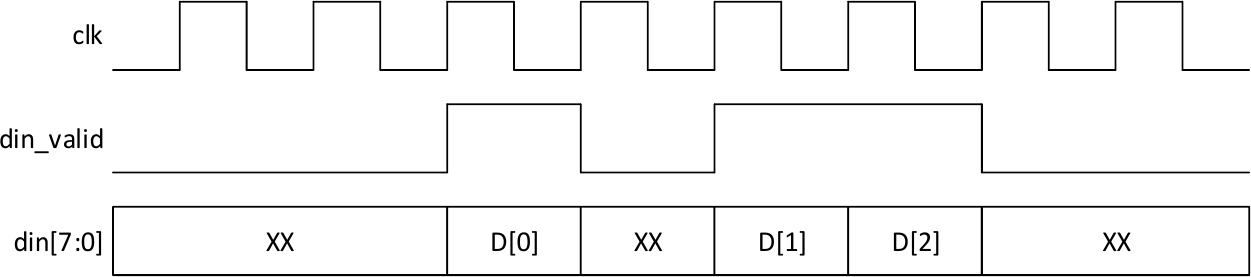
\includegraphics[width=1\textwidth]{din}
        \caption{Input}
        \label{fig:input_expected_waveform}
        \vspace*{.6cm}
    \end{subfigure}
    \begin{subfigure}{.95\textwidth}
        \centering
        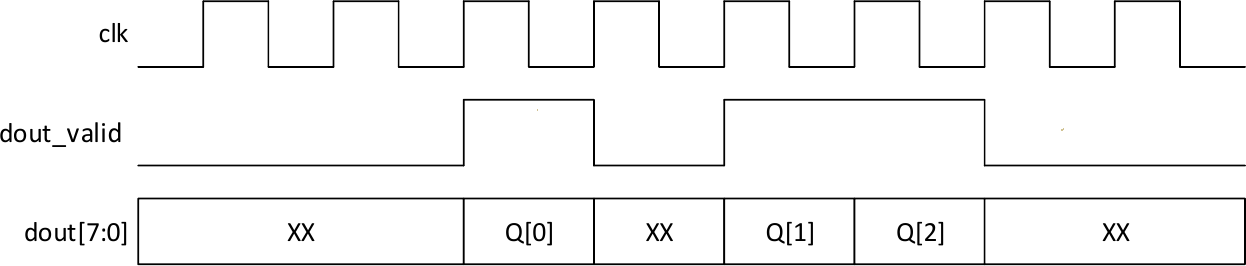
\includegraphics[width=1\textwidth]{dout}
        \caption{Output}
        \label{fig:output_expected_waveform}
    \end{subfigure}
    \caption{Expected waveforms}
    \label{fig:expected_waveforms}
\end{figure}\clearpage
\section{Design choices}
In this section we will present the design choices. First, notice that the stream cipher module shall be reset before its usage. Whenever the reset signal is asserted, other signals are ignored. Reset is negedge triggered.

Secondly, all the logic of the stream cipher module (except the S-box) is synchronous.

\subsection{S-box}
We have implemented the S-box in a separate module with respect to the stream cipher for higher reusability and to respect the Single Responsibility Principle.

In particular, we have implemented it as a lookup-table in continuous assignment. The S-box is defined as a packed two-dimensions array:
\begin{lstlisting}
wire [0:255][7:0] sbox;
\end{lstlisting}
S-box elements have been assigned in continuous assignments as following:
\begin{lstlisting}
assign sbox[8'h00] = 8'h63;
assign sbox[8'h01] = 8'h7c;
/* other 254 assignments... */
\end{lstlisting}
The module takes an input of 8-bits and outputs the result of the lookup as an 8-bit value. This is done in a continuous assignment too:
\begin{lstlisting}
assign out = sbox[in];
\end{lstlisting}

\subsection{Key management}

To keep the key correctly stored inside the module, we use an internal counter block (\lstinline{cb}), which is defined as an 8-bit reg.

On reset, the counter block is set to zero as a default value. An additional 1-bit input signal (\lstinline{key_in}) has been added to allow to set the key. To correctly set the key, the \lstinline{key} signal must contain the key and must be stable, and the \lstinline{key_in} signal must be asserted. When these conditions are met, the key will be saved into the internal counter block \lstinline{cb} at the next rising edge of the clock. Moreover, there will be no output the next clock cycle, therefore we also deassert the \lstinline{dout_valid} signal.

\subsection{Hardware logic}
When the 1-bit \lstinline{din_valid} signal is asserted, the 8-bit input signal \lstinline{din} must to be valid and stable. The \lstinline{din} signal value is XORed with the result of the lookup in the S-box of the counter block \lstinline{cb} and it is stored in \lstinline{dout} and \lstinline{dout_valid} is asserted. If \lstinline{din_valid} is not asserted, \lstinline{dout_valid} is deasserted. The \lstinline{dout} signal shall not be considered when \lstinline{dout_valid} is deasserted, as per specification.

Every clock cycle, if \lstinline{din_valid} is asserted (and \lstinline{key_in} is not), the counter block is increased by one modulo $256$. Notice that the modulo addition is implemented as a simple sum on an 8-bit reg, which implicitly overflows (without any warning or error generated from used tools). We decided to implement it this way because we found out that it performed better (about $5 MHz$ increase) with respect to other implementations.

\clearpage
\section{Block diagram}
The top-level view of our module is represented in \cref{fig:top_level}, with every input and output.

\lstset{basicstyle=\large\ttfamily}
\begin{figure}[!ht]
    \centering
    \begin{circuitikz}
        \tikzset{box/.style = {draw=black, thick,minimum height=5cm, text width=5cm,align=center}}
        \node (GCR) [box] {\parbox{4cm}{\Large\centering AES S-box based\\stream cipher}};

        \draw ($(GCR.south west)!1!(GCR.south)$) -- ++(0,-.5) node[anchor=north]{\lstinline{clk}};
        \draw ($(GCR.south west)!1!(GCR.south)$) ++(-.25,0.01) -- ++(0.25,0.25);
        \draw ($(GCR.south west)!1!(GCR.south)$) ++(.25,0.01) -- ++(-0.25,0.25);

        \draw [<-,>=stealth]($(GCR.north west)!.3!(GCR.west)$) -- ++(-1,0) node[anchor=east]{\lstinline{din}};
        \draw [<-,>=stealth]($(GCR.north west)!.6!(GCR.west)$) -- ++(-1,0) node[anchor=east]{\lstinline{din_valid}};
        \draw [<-,>=stealth]($(GCR.north west)!.9!(GCR.west)$) -- ++(-1,0) node[anchor=east]{\lstinline{key}};
        \draw [<-,>=stealth]($(GCR.north west)!1.2!(GCR.west)$) -- ++(-1,0) node[anchor=east]{\lstinline{key_in}};
        \draw [<-,>=stealth]($(GCR.north west)!1.7!(GCR.west)$) -- ++(-1,0) node[anchor=east]{\lstinline{rst_n}};

        \draw [->,>=stealth]($(GCR.north east)!0.75!(GCR.east)$) -- ++(1,0) node[anchor=west] {\lstinline{dout}};
        \draw [->,>=stealth]($(GCR.north east)!1.25!(GCR.east)$) -- ++(1,0) node[anchor=west] {\lstinline{dout_valid}};
    \end{circuitikz}
    \caption{Top-level view of the AES S-box based stream cipher}
    \label{fig:top_level}
\end{figure}
\lstset{basicstyle=\small\ttfamily}

We are now going to describe the synthesized netlist in all of its parts. For the full picture, please refer to the next page.

The update of the counter block \lstinline{cb} is implemented with a simple adder, where the result is used only when \lstinline{din_valid} is asserted. However, if \lstinline{key_in} is asserted, the update for the counter block register \lstinline{cb} is taken from the \lstinline{key}signal.
\begin{figure}[!ht]
    \centering
    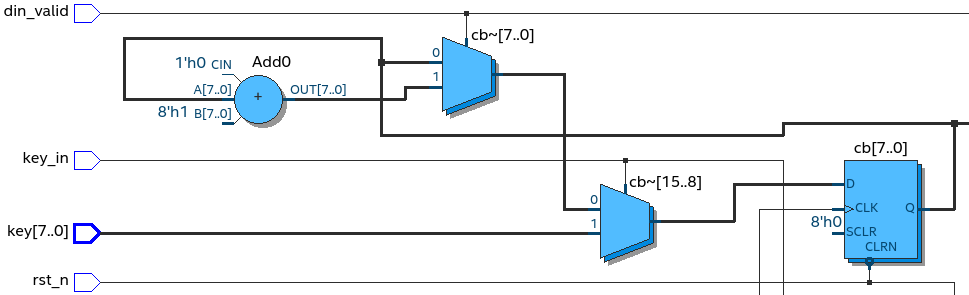
\includegraphics[width=1\textwidth]{key_manage_netlist}
    \caption{Key management}
    \label{fig:key_manage_netlist}
\end{figure}

\clearpage
\newgeometry{top=0pt, bottom=0pt, left=0pt, right=0pt}
\begin{figure}
    \thispagestyle{empty}
    \centering
    \hspace*{-9cm}
    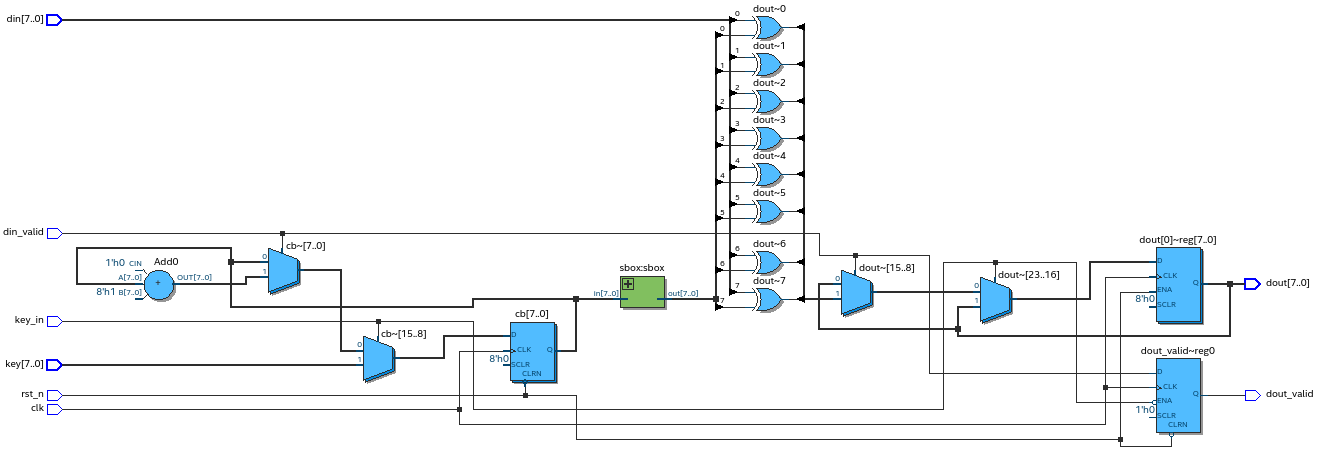
\includegraphics[width=1\textheight, angle=90]{complete_netlist}
\end{figure}
\restoregeometry
\clearpage

The S-box (\cref{fig:sbox_netlist}) is implement with 8 multiplexer in parallel with an 8-bit selection signal.
\begin{figure}[!ht]
    \centering
    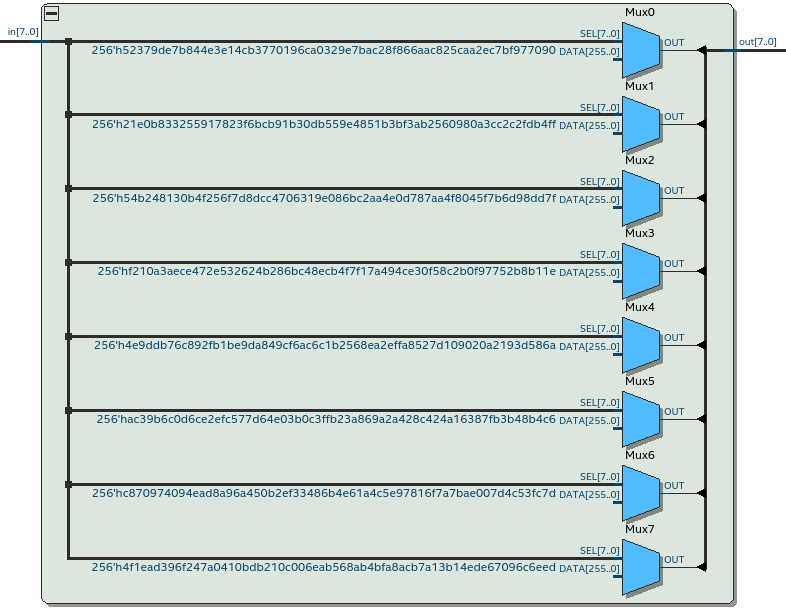
\includegraphics[width=1\textwidth]{sbox_netlist}
    \caption{S-box netlist}
    \label{fig:sbox_netlist}
\end{figure}

The encryption (\cref{fig:encryption_netlist}) is a simple XOR cascade where the inputs are the \lstinline{din} signal value and the output value of the S-box lookup.
\begin{figure}
    \centering
    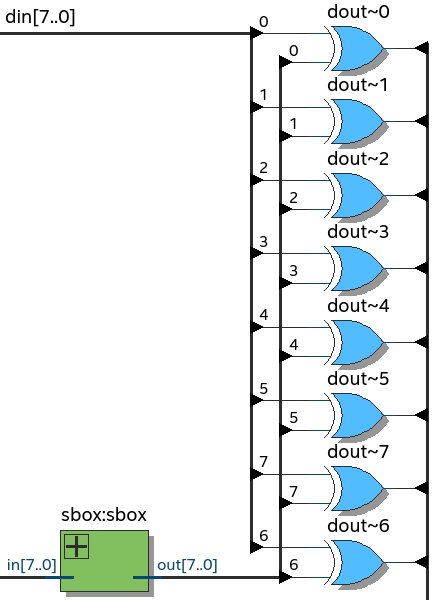
\includegraphics[width=.5\textwidth]{encryption_netlist}
    \caption{Encryption netlist}
    \label{fig:encryption_netlist}
\end{figure}

Finally, we have the output handling (\cref{fig:output_netlist}). The \lstinline{key_in} signal and the \lstinline{din_valid} signal control whether to update \lstinline{dout} with a new value or to keep the old one. This is done by selecting the multiplexers input line. When the \lstinline{key_in} signal is asserted, the \lstinline{dout_valid} signal gets deasserted.
\begin{figure}
    \centering
    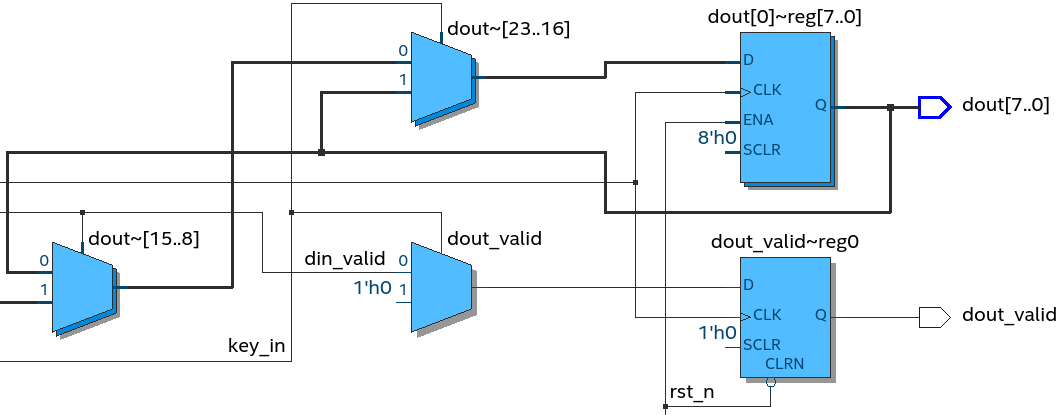
\includegraphics[width=1\textwidth]{output_netlist}
    \caption{Output netlist}
    \label{fig:output_netlist}
\end{figure}\clearpage
\section{Waveforms}\clearpage
\section{Testbench}
\label{sec:tests}
We will now describe the tests that were conducted on the designed hardware module.

\begin{enumerate}
    \item Given that the key space is small enough\footnote{Actually, the key space is definitely too small to provide any security.}, we are able to completely test the encryption (or, symmetrically, the decryption) of our module. Hence, a test performs the encryption of every possible character ($2^8$ possible characters) with every possible key ($2^8$ possible values).
    \item We have repeated the first test, but adding a random number (0 to 5) of idle cycles between the encryption of two values. This test was carried out to check that the signals were properly handled by our module.
    \item Finally, we have checked that the \cref{thm:enc_inv_dec} actually holds. To do so, we have encrypted a file ($\sim$39000 characters), and subsequently we have checked that its decryption (using the same key) was the same as the original file.
\end{enumerate}\clearpage
\section{RTL}\clearpage
\section{Static Timing Analysis}

\end{document}
